\documentclass[pdftex,12pt,a4paper]{article}
\usepackage[pdftex]{graphicx}
\usepackage{xcolor}
\usepackage{marginnote}
\usepackage{enumitem}
\usepackage[bottom=1.5cm, outer=5cm, inner=2cm, heightrounded,
marginparwidth=4cm, marginparsep=0.5cm]{geometry}

\begin{document}
    % Custom title page
    \begin{titlepage}
        \begin{center}
            
\includegraphics[width=5cm]{figures/kulogo}\\[1cm]
            {\Large \bfseries
                Spring 2014\\
                Computer Networks\\
                CMPE323\\[1cm]
            }
            {\large \bfseries
                \noindent Laboratory Experiment No. 2: Introduction to Ethernet
                Networks\\[1cm]
            }
        \end{center}

        \noindent \textbf{Aims and Objectives:}
            \begin{itemize}[leftmargin=4cm]
                \item Introduce students to layer 2 aspects of Ethernet,
                \item the structure of Ethernet frames,
                \item the functionality of broadcast domains,
                \item foresee the scalability issues of broadcast domains,
                \item and basic protocol analysing techniques.
            \end{itemize}
            \vspace{0.5cm}

        \noindent \textbf{Materials Required:}
            \begin{itemize}[leftmargin=4cm]
                \item Ethernet switches,
                \item PCs with Ethernet adapters,
                \item and Straight-through/crossover/rollover cables.
            \end{itemize}
            \vspace{0.5cm}

        \noindent \textbf{Change Log:}
            \begin{itemize}[leftmargin=4cm]
                \item 23-2-2014: original document -- mkhonji.
            \end{itemize}
    \end{titlepage}
    \newpage

    % Lab script content
    \section{Introduction}
        Ethernet (specified in the standard IEEE 802.3) is a set of protocols
        that facilitate communication among devices over Local Area Networks
        (LANs).  Such protocols span the OSI layers 1 and 2. For example, the
        standard IEEE 802.3 specification includes (not limited to):
        \begin{itemize}
            \item layer 1 specifications (e.g. cable specifications, line
            coding method\footnote{Basically, line coding methods (e.g.
            Manchester encoding) can describe how to signal bits of 0s and 1s
            to a remote end by transitioning voltage over a medium such as the
            copper wires in Cat5e cables that are available in the lab.}),
            \item and layer 2 specifications (e.g. MAC frames, LLC).
        \end{itemize}
        
        However, this lab will only focus on the most-widely used layer 2
        aspects of Ethernet. Layer 1 details will be omitted as they are closer
        to electrical engineering and communications than the subjects of
        CMPE323 labs.

        \subsection{High-level overview of Ethernet networks}
            For simplicity, this lab is focused on common layer 2 aspects of
            Ethernet II only, which is the most wide-spread Ethernet type.
            \begin{itemize}
                \item When nodes (e.g. PCs) transmit data over the network, the
                data must be encapsulated in a packet that is formatted
                according to Figure \ref{fig:macpacket}. \textbf{Note:} the
                hardware (e.g. Ethernet NICs) handle the fields
                \texttt{PREAMBLE}, \texttt{SFD}, \texttt{FRAME CHECK SEQUENCE}
                transparently and does not pass them to the upper software
                layers (the Operating System (OS) cannot see those fields). The
                same applies when sending messages, there is no need to adds
                the named fields earlier in any system call as the hardware
                layer will add them too. In other words, we need to only send
                the fields that are marked as \emph{frame} (as the hardware
                will add the surrounding \emph{packet} fields automatically,
                which we cannot disable with normal NICs that we have in our
                lab).

                \begin{figure}[tbh]
                    \centering
                    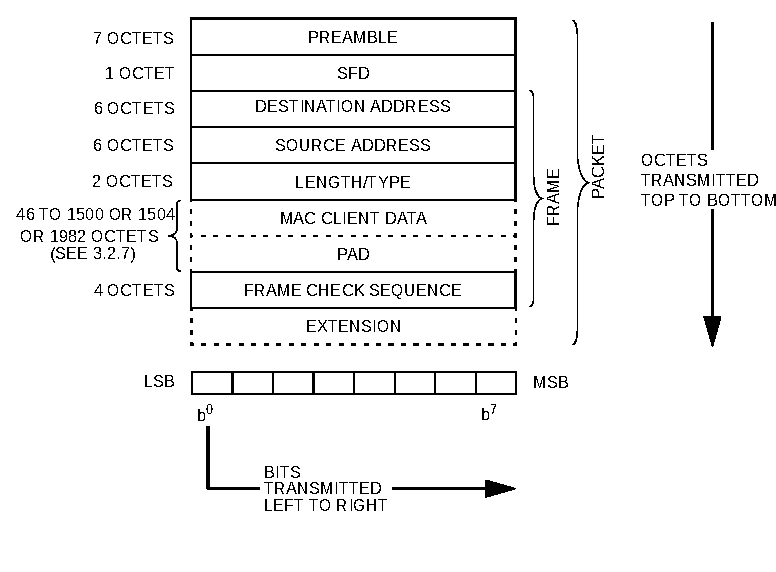
\includegraphics[width=0.9\textwidth]{figures/macpacket}
                    \caption{Ethernet Media Access Control (MAC) packet. Note:
                    an octet is 8 bits --- Source: IEEE Std. 802.3-2012.}
                    \label{fig:macpacket}
                \end{figure}

                \item This packet encapsulation facilitates a number things,
                most importantly:
                    \begin{itemize}
                        \item The ability to specify which target node (e.g.
                        PC) should receive the data.  This is possible since
                        each Ethernet NIC in a PC has a unique address called
                        the \emph{MAC Address} and that intermediate Ethernet
                        switches forward such Ethernet packets based on these
                        addresses,
                        \item the ability to specify the protocol\footnote{The
                        \emph{Length/Type} field can be either used for the frame's
                        length (in bytes) by which an LLC header is required,
                        or the payload's protocol type as in Ethernet II (which
                        this lab is about).} by
                        which the payload data is formatted as. This allows the
                        receiver node to know how to interpret the Ethernet
                        frame data payload,
                        \item A checksum value to allow the receiver to
                        determine whether a received MAC frame has any
                        errors\footnote{Examples of errors could be the change
                        of a bit of (say) 1 into a 0 due to electromagnetic
                        interference that could be caused by electrical devices
                        around the copper medium (as in our Cat5e cables).}.
                    \end{itemize}
                
                \item When an Ethernet switch receives a MAC packet, it
                generally performs the following tasks:
                    \begin{itemize}
                        \item Populates its local MAC address table:
                            \begin{enumerate}
                                \item For every MAC packet that enters the switch, the
                                switch reads the source MAC address and adds an entry
                                in its MAC address table that maps the source MAC
                                address to the port identifier by which the
                                corresponding MAC packet entered the switch.
                            \end{enumerate}
                        \item Forwards the MAC packet:
                            \begin{enumerate}
                                \item For every MAC packet that enters the switch, the
                                switch reads the destination MAC address from the MAC
                                packet.
                                \item If the destination MAC address is
                                \texttt{FF:FF:FF:FF:FF:FF} (in hex), the switch will
                                forward the received MAC packet to all of its
                                ports except the one from which it received the
                                packet (i.e. broadcasting).
                                \item For other MAC addresses, the switch looks
                                up its MAC address table\footnote{The MAC
                                address table basically contains entries that
                                map MAC addresses to local Ethernet switch
                                ports that lead to the node with the given MAC
                                address.}. If the Ethernet switch finds an entry in the MAC
                                address table, it will forward the MAC packet only to the
                                Ethernet port associated with that entry. Else,
                                it will forward the MAC packet to all of its
                                ports (except the one it received the MAC
                                packet from).
                            \end{enumerate}
                    \end{itemize}
            \end{itemize}

    \section{Lab Preparation}
        \begin{itemize}
            \item Connect PCs to an Ethernet switch as depicted in Figure
            \ref{fig:netdiag}.
                \begin{figure}[tbh]
                    \centering
                    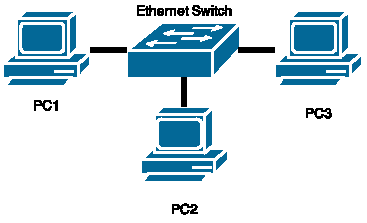
\includegraphics[width=0.5\textwidth]{figures/netdiag}
                    \caption{Experiment's physical topology.}
                    \label{fig:netdiag}
                \end{figure}
            \item Erase any configuration from the switch:
                \begin{enumerate}
                    \item Connect the switch's console port to your PC's serial port
                    using the provided roll-over cable (ask the lab engineer
                    for help).
                    \item If you are using Windows, use HyperTerm or Putty to
                    connect to the serial port of your PC. If you are using a
                    Linux distribution, execute the following command
                    \texttt{screen /dev/ttySx} Where \texttt{x} is the ID of
                    the serial port that you have connected the console port
                    to.
                    \item Once connected to the switch via the serial port
                    (using \texttt{screen} or whatever Windows alternative),
                    execute the following commands:
                        \begin{enumerate}
                            \item \texttt{enable} \textcolor{gray}{// to
                            activate privileged mode.}
                            \item \texttt{erase startup-config}
                            \textcolor{gray}{// to delete previous
                            configurations.}
                            \item \texttt{reload} \textcolor{gray}{// to reboot
                            the switch. Submit \texttt{N} when asked to save
                            the configuration}
                        \end{enumerate}
                \end{enumerate}
            \item Run the protocol analyzer application \emph{Wireshark} on all
            of the three PCs. You can do this by either following the GUI's
            menus or by simply executing the command \texttt{wireshark} in a
            terminal.
        \end{itemize}

    \section{Lab Experiments}
        \subsection{Send your 1$^{st}$ manually-crafted MAC packet from PC1
        $\longrightarrow$ PC3}\label{sec:1to3}
            \begin{flushright}
                \textbf{[33 points]}\marginnote{\small \textbf{Note:} when done, show your
                work to the the lab engineer for grading purposes.}
            \end{flushright}

            \begin{enumerate}
                \item View\footnote{You can view the MAC address table of a
                Cisco switch by executing the command \texttt{show mac-address
                table} in the privileged mode.} the MAC address table of the
                switch, and note down the \emph{dynamic} MAC address entries in
                the table.

                \item From PC1, send\footnote{You can send such low-level
                messages using \texttt{scapy}'s \texttt{sendp} command as
                follows:
                \texttt{sendp('\textbackslash x11\textbackslash
                x11\textbackslash x11\textbackslash x11\textbackslash
                x11\textbackslash x11\textbackslash x33\textbackslash
                x33\textbackslash x33\textbackslash x33\textbackslash
                x33\textbackslash x33\textbackslash x05\textbackslash
                xFF\textbackslash x48\textbackslash x65\textbackslash
                x6C\textbackslash x6C\textbackslash x6F')}} the following message: 
                    \begin{itemize}
                        \item Source MAC address (6 bytes in hex):
                        \texttt{11:11:11:11:11:11}.
                        \item Destination MAC address (6 bytes in hex):
                        \texttt{33:33:33:33:33:33}.
                        \item EtherType\footnote{Named as \emph{Type/Length} in
                        Figure \ref{fig:macpacket}.}: \texttt{0x05FF}
                        \marginnote{\textbf{Note:} for the purpose of this
                        task, you can choose any 2 byte value for EthType.
                        However, we suggest \texttt{0x05FF} as it is not
                        assigned to any protocol so that Wireshark won't
                        attempt to parse the payload once you capture it (for
                        visual clarity).}
                        \item Message payload: ``Hello'' (in hex: \texttt{0x48,
                        0x65, 0x6c, 0x6c, 0x6f}).
                    \end{itemize}

                \item Once you send the message above, answer the following:
                    \begin{itemize}
                        \item Did the message appear on PC3's Wireshark
                        instance?
                        \item Did the message appear on PC2's Wireshark
                        instance?
                        \item View the MAC address table of the switch again,
                        do you see any new added addresses? 
                        \item What is the newly added MAC address entry in the
                        MAC address table?
                        \item What interface is the new MAC addressed mapped
                        to?
                    \end{itemize}
            \end{enumerate}

        \subsection{Send your 1$^{st}$ manually-crafted MAC packet from PC3
        $\longrightarrow$ PC1}\label{sec:3to1}
            \begin{flushright}
                \textbf{[33 points]}\marginnote{\small \textbf{Note:} When done, show your
                work to the the lab engineer for grading purposes.}
            \end{flushright}

            \begin{enumerate}
                \item From PC3, send the follows back to PC1's MAC address:
                    \begin{itemize}
                        \item Source MAC address (6 bytes in hex):
                        \texttt{33:33:33:33:33:33}.
                        \item Destination MAC address (6 bytes in hex):
                        \texttt{11:11:11:11:11:11}\marginnote{\textbf{Note:} the same
                        MAC addresses that PC1 used earlier. Recall the added
                        entry in the MAC address table?}
                        \item EtherType: \texttt{0x05FF}
                        \item Message payload: ``Hello'' (in hex: \texttt{0x48,
                        0x65, 0x6c, 0x6c, 0x6f}).
                    \end{itemize}

                \item Once you send the message above, answer the following:
                    \begin{itemize}
                        \item Did the message appear on PC1's Wireshark
                        instance?
                        \item Did the message appear on PC2's Wireshark
                        instance?
                        \item View the MAC address table of the switch again,
                        do you see any new added addresses? 
                        \item What is the newly added MAC address entry in the
                        MAC address table?
                        \item What interface is the new MAC addressed mapped
                        to?
                    \end{itemize}
            \end{enumerate}

        \subsection{Logical conclusions}
            \begin{flushright}
                \textbf{[34 points]}\marginnote{\small \textbf{Note:} When done, show your
                work to the the lab engineer for grading purposes.}
            \end{flushright}

            Based on the experiments that you have performed earlier, answer
            the following questions:
            \begin{itemize}
                \item How do Ethernet networks identify its nodes (or PCs)? In
                other words, how can the Ethernet network know which node you
                wish to send your MAC packet to?
                \item If an Ethernet switch receives a MAC packet from its
                interface $X$, and the destination MAC address that does not
                exist in its MAC address table, then:
                    \begin{itemize}
                        \item How would the switch update the MAC address
                        table?
                        \item How would the switch forward the packet?
                    \end{itemize}
                \item If an Ethernet switch receives a MAC packet with a
                destination MAC address that does indeed exist in its MAC address
                table such that it is mapped to some interface $X$, how would
                the switch forward the packet?
                    \begin{itemize}
                        \item How would the switch forward the packet?
                    \end{itemize}
                \item Suppose that you have 1,000,000 nodes (or PCs) connected
                to a set of connected switches forming a single broadcast
                domain, also suppose that all of the nodes have unique MAC
                addresses and are communicating with each other. How many MAC
                addresses do you expect to exist in each Ethernet switch?
            \end{itemize}

        \subsection{Bonus questions (not graded)}\marginnote{\small
        \textbf{Note:} when done, show your answers to the lab engineer for
        feedback. If the lab time is not enough, take your time and submit it
        in a later time. Although not graded, it can strengthen your
        understanding of the subject.}
            Based on the behaviour that you saw in earlier experiments, below
            are additional interesting questions that you are encouraged to
            think about (and answer):
            \begin{itemize}
                \item What do you think are the possible outcomes if we connect
                the 1,000,000 actively inter-communicating nodes to a set of switches
                were one of the switches has a maximum capacity of storing 500
                MAC addresses only?
                \item How would the switch behave if its MAC address table is
                full?
                \item Repeat the experiments \ref{sec:1to3} and \ref{sec:3to1}
                except for replacing the MAC address of PC1 to
                \texttt{FF:FF:FF:FF:FF:FF}. What is the difference? Do you
                notice anything special with this address?
            \end{itemize}
\end{document}
